\documentclass[10pt,a4paper]{article}
\usepackage[utf8]{inputenc}
\usepackage[english]{babel}
\usepackage{amsmath}
\usepackage{amsfonts}
\usepackage{amssymb}
\usepackage{graphicx}
\usepackage[left=2cm,right=2cm,top=2cm,bottom=2cm]{geometry}
\usepackage{cite}
\usepackage{xspace}

\usepackage{hyperref}


\usepackage{xcolor}
\usepackage{mdframed}

\usepackage{caption}
\usepackage{subcaption}

% listings
\usepackage{listings}
\definecolor{codegreen}{rgb}{0,0.6,0}
\definecolor{codegray}{rgb}{0.5,0.5,0.5}
\definecolor{codepurple}{rgb}{0.58,0,0.82}
\definecolor{backcolour}{rgb}{0.95,0.95,0.92}

\lstdefinestyle{code}{
    backgroundcolor=\color{backcolour},   
    commentstyle=\color{codegreen},
    keywordstyle=\color{magenta},
    numberstyle=\tiny\color{codegray},
    stringstyle=\color{codepurple},
    basicstyle=\ttfamily\footnotesize,
    breakatwhitespace=false,         
    breaklines=true,                 
    captionpos=b,                    
    keepspaces=true,                 
    numbers=left,                    
    numbersep=5pt,                  
    showspaces=false,                
    showstringspaces=false,
    showtabs=false,                  
    tabsize=2
}
\lstdefinestyle{plain}{
    %backgroundcolor=\color{backcolour},   
    commentstyle=\color{codegreen},
    keywordstyle=\color{magenta},
    numberstyle=\tiny\color{codegray},
    stringstyle=\color{codepurple},
    basicstyle=\ttfamily\footnotesize,
    breakatwhitespace=false,         
    breaklines=true,                 
    captionpos=b,                    
    keepspaces=true,                 
    %numbers=left,                    
    numbersep=5pt,                  
    showspaces=false,                
    showstringspaces=false,
    showtabs=false,                  
    tabsize=2
}

\lstset{style=plain}

% TikZ
\usepackage{tikz,xstring,siunitx,pgfplots}
\usepackage[american,europeancurrent,europeanvoltage,siunitx]{circuitikz}
\ctikzset{bipoles/length=1.4cm}
\usetikzlibrary{shapes,arrows}
\usetikzlibrary{calc,patterns,decorations.pathmorphing,decorations.markings}
\usetikzlibrary{circuits,circuits.ee.IEC}
\usetikzlibrary{pgfplots.groupplots}
\usetikzlibrary{backgrounds}
\usetikzlibrary{matrix, positioning, fit}


\DeclareMathOperator{\diag}{diag}
\DeclareMathOperator{\atan}{atan}
\newcommand{\bs}[1]{\boldsymbol{\mathrm{#1}}}
\newcommand{\course}{Introduction to Applied AI\xspace}
\newcommand{\courseCode}{DVA132\xspace}

\begin{document}
\begin{mdframed}
\begin{center}
\textbf{\course (\courseCode)}\\
\textbf{Report Assignment Clustering}\\
\textbf{Your Name, Student-ID}\\    %Insert your name and student-ID
\textbf{\today}
\end{center}
\end{mdframed}

\begin{figure}[htb]
	\centering
	\begin{subfigure}[b]{0.3\textwidth}
	    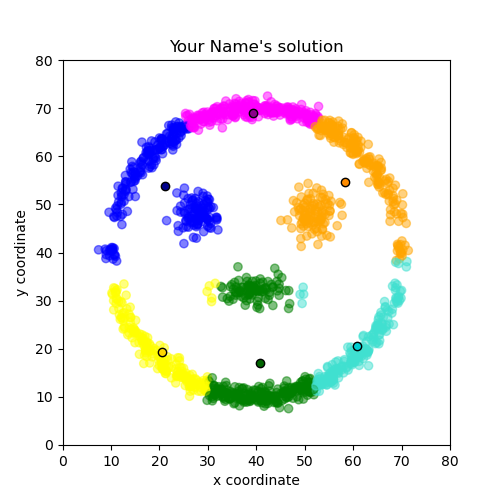
\includegraphics[width=\textwidth]{clustering_solution.png} %insert your K-means solution image for dataset 1
	    \caption{Dataset 1 -- K-means}
	    \label{fig:kmeans}
	\end{subfigure}
	\begin{subfigure}[b]{0.3\textwidth}
	    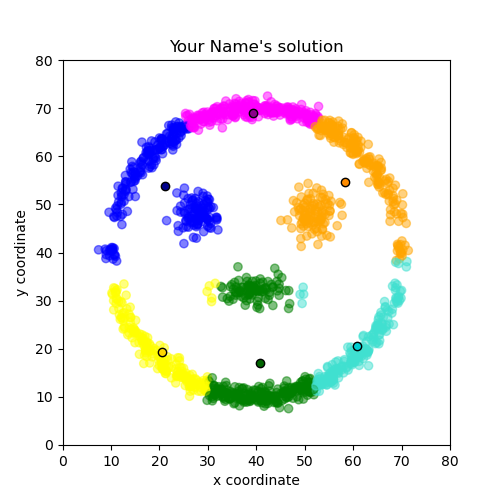
\includegraphics[width=\textwidth]{clustering_solution.png} %insert your DBSCAN solution 1 image 
	    \caption{Dataset 2 --- DBSCAN 1}
	    \label{fig:dbscan4}
	\end{subfigure}
	\begin{subfigure}[b]{0.3\textwidth}
	    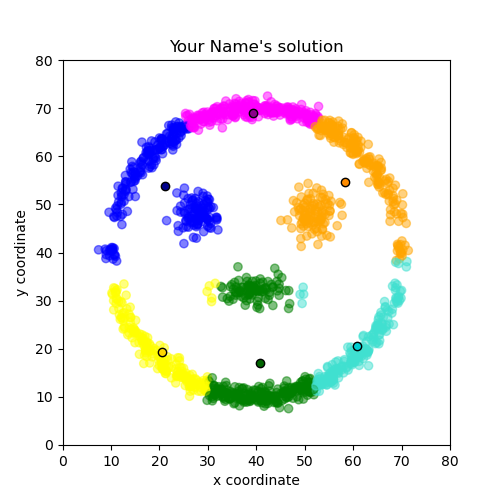
\includegraphics[width=\textwidth]{clustering_solution.png} %insert your DBSCAN solution 2 image
	    \caption{Dataset 2 --- DBSCAN 2}
	    \label{fig:dbscan7}
	\end{subfigure}
	\caption{Clustering solutions}
	\label{fig:solution}
\end{figure}

\begin{mdframed}
K-means:
    \begin{itemize}
        \item Dataset1, Figure~\ref{fig:kmeans}:
        \begin{itemize}
            \item K = 1 %insert your K
        \end{itemize}
        \item Dataset2        
        \begin{itemize}
            \item K = 1 %insert your K
        \end{itemize}
        \item Reason for K-means to fail: %insert your own comment/thoughts
    \end{itemize}
DBSCAN:
    \begin{itemize}
        \item Dataset2 solution 1, Figure~\ref{fig:dbscan4}:
        \begin{itemize}
            \item R = 10 %insert R
            \item minPoints = 2 %insert minPoints
        \end{itemize} 
        \item Dataset2 solution 2, Figure~\ref{fig:dbscan7}
        \begin{itemize}
            \item R = 10 %insert R
            \item minPoints = 2 %insert minPoints
        \end{itemize} 
    \end{itemize}
\end{mdframed}



\end{document}